\documentclass[11pt]{beamer}
\usetheme{Singapore}
\usepackage[utf8]{inputenc}
\usepackage[french]{babel}
\usepackage[T1]{fontenc}
\usepackage{amsmath}
\usepackage{amsfonts}
\usepackage{amssymb}
\author{Le groupe MkRpg}
\title{Présentation du projet MkRpg}
%\setbeamercovered{transparent} 
\setbeamertemplate{navigation symbols}{} 
\renewcommand{\insertnavigation}[1]{\hfill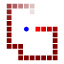
\includegraphics[scale=.5]{main.png}~\vspace{-.2cm}}
% Raoul :
%\renewcommand{\insertnavigation}[1]{\hfill
\includegraphics[scale=.25]{raoul.png}~\vspace{-.2cm}}
%\setbeamertemplate{headline}{}
%\logo{} 
%\institute{} 
%\date{} 
%\subject{} 
\begin{document}

\begin{frame}{Architecture}
	\begin{center}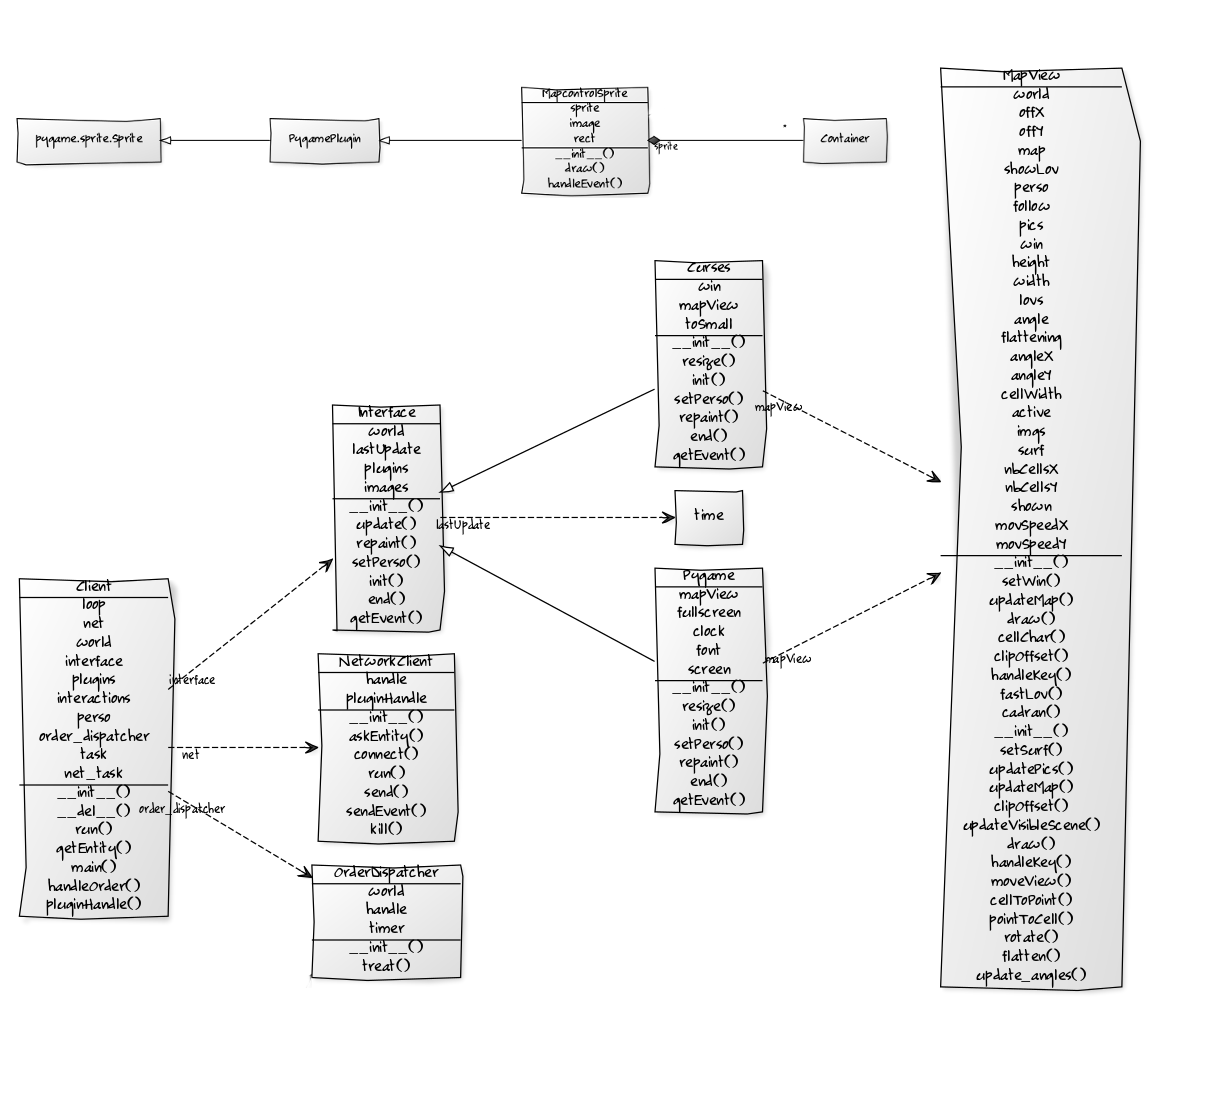
\includegraphics[scale=0.21]{uml_pygame.png}\end{center}
\end{frame}

\begin{frame}{Interface pygame : features}
	\begin{itemize}
		\item mise en cache
    \item changement de cartes
    \item rotation de carte
    \item zoom/dezoom
    \item affichage d'objets
    \item système de gui
    \item plugins d'affichage
	\end{itemize}
\end{frame}

\begin{frame}{Interface pygame}
	\begin{itemize}
    \item performances : raisonnables, 30 FPS, quelques lags quand on affiche des parties trop importantes de la map
		\item[]
    \item stabilité : quelques exceptions non capturées (rotation de carte), sinon affichage très stable
	\end{itemize}
\end{frame}

\begin{frame}{Interface pygame}
	\begin{center}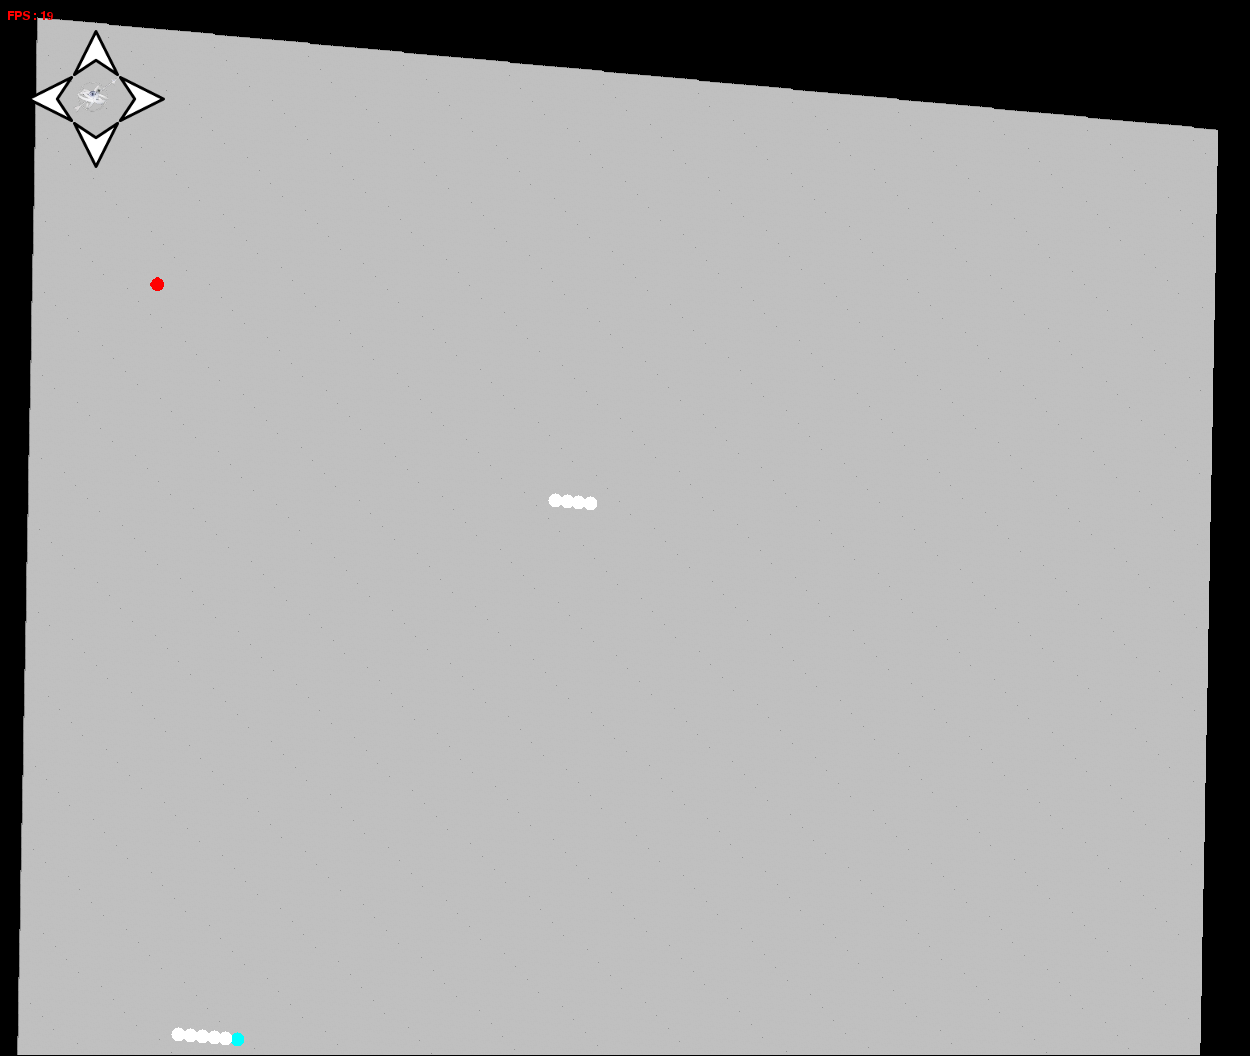
\includegraphics[scale=0.2]{game_screenshot.png}\end{center}
\end{frame}

\begin{frame}{Continuité du projet : interface pygame}
	\begin{itemize}
		\item architecture de l'interface cohérente et pratique
		\item système de plugin tout puissant (tout est modifiable à travers des plugins)
		\item[]
		\item interface soutenable a moyen terme pour des jeux de taille moyenne
	\end{itemize}
\end{frame}

\begin{frame}{Remarques : pygame}
	\begin{itemize}
		\item efficace pour de petits projets
		\item pas adapté aux moyens/gros projets
		\item quelques problèmes de compatibilité
		\item manque de documentation avancée et/ou d'exemples d'utilisation avancés suffisamment commentés
	\end{itemize}
\end{frame}

\begin{frame}{Remarques : projet}
	\begin{itemize}
		\item on a sous-estimé la charge de travail liée à l'affichage
		\item[]
		\item quelques problèmes de communication en cours de route
		\item gros problème de partage des taches malgré quelques tentatives pour mieux les répartir
		\item[]
		\item difficile à tester
	\end{itemize}
\end{frame}
\end{document}
